\documentclass[twocolumn]{article}
\usepackage[T1]{fontenc}
\usepackage{times}
\usepackage{mathptmx}
\usepackage{listings}
\usepackage[scaled=0.88]{luximono}
\usepackage{tikz}
\usepackage{booktabs}
\usepackage{array}
\usetikzlibrary{matrix,arrows,positioning,automata}
%\usetikzlibrary{automata}
\tikzset{>=latex}
\lstset{language=C,
  basicstyle={\ttfamily},
}
\usepackage{graphicx}

% http://hackingoff.com/compilers/regular-expression-to-nfa-dfa
% http://jsmachines.sourceforge.net/machines/slr.html

\usepackage[left=2pc,right=8pc,top=4pc,bottom=4pc]{geometry}

\title{COMS W4115 Programming Languages and Translators \\
Homework Assignment 2 Solutions}
\author{Prof. Stephen A. Edwards}
\date{}

\pagestyle{empty}

% Make | a mathrel symbol: improves alternation (a | b) spacing
\mathcode`\|="326A


\def\kleene#1#2#3#4{
\path [->] 
      (#1) edge node [above] {$\epsilon$} (#2)            
      (#3) edge node [above] {$\epsilon$} (#4)
      (#1) edge [bend right=50, looseness=1] node [below] {$\epsilon$} (#4)
      (#3) edge [bend right=85, looseness=1.2] node [above] {$\epsilon$} (#2)
;
}
\def\choice#1#2#3#4#5#6{
\path [->] 
      (#1) edge node [above left] {$\epsilon$} (#2)            
      (#1) edge node [below left] {$\epsilon$} (#3)
      (#4) edge node [above right] {$\epsilon$} (#6)            
      (#5) edge node [below right] {$\epsilon$} (#6)
;
}

\begin{document}
\maketitle
\thispagestyle{empty}

\raggedright


\begin{enumerate}


\item Write a regular expression for floating point literals according
  to the following (after K\&R):

\begin{quote}
A floating constant consists of an integer part, a decimal point, a
fraction part, an \texttt{e} or an \texttt{E}, and an optionally
signed integer exponent. The integer and fraction parts both consist
of a sequence of digits. Either the integer part, or the fraction part
(not both) may be missing; either the decimal point or the
\texttt{e}/\texttt{E} and the exponent (not both) may be missing.
\end{quote}

\begin{verbatim}
let Exp = ('e' | 'E') ('+'|'-')? [0-9]+
 
(          '.' [0-9]+ Exp?
| [0-9]+ ( '.' [0-9]* Exp?
                    | Exp))
\end{verbatim}

\item Draw a DFA for a scanner that recognizes and distinguishes the
  following set of keywords.  Draw accepting states with double lines
  and label them with the name of the keyword they accept.  Follow the
  definition of a DFA given in class.

\noindent
\texttt{deinit fileprivate func open operator private if init self Self Any as}

\begin{figure}[t]
  \centerline{\includegraphics[width=0.5\columnwidth]{hw2-2.pdf}}
\end{figure}

% http://hackingoff.com/compilers/regular-expression-to-nfa-dfa



\item Construct NFAs and DFAs for the regular expressions:

\def\n#1{\node (#1) {#1};}
\def\nn#1{\node [double] (#1) {#1};}
\def\arc#1#2#3{\draw [->] (#1) edge node {$#3$} (#2);}
\def\arcl#1#2#3{\draw [->] (#1) edge node [left] {$#3$} (#2);}
\def\arcb#1#2#3{\draw [->] (#1) edge [bend left=10] node {$#3$} (#2);}

\begin{enumerate}

  \item  $a\ (a^* | b^*)\ a$

\begin{tikzpicture}[auto]
\matrix [every node/.style={circle,draw},
         column sep=1pc,
         row sep=1pc,
         execute at begin cell=\n,
         execute at end cell=,
         execute at empty cell=] {
 & &2&3&4&5\\
0&1& & & & &{10}&{11}\nn{11}\\
 & &6&7&8&9\\
}
;
\arc 0 1 a
\choice 1 2 6 5 9 {10}
\arc 3 4 a
\arc 7 8 b
\arc {10} {11} a
\kleene 2 3 4 5
\kleene 6 7 8 9
\end{tikzpicture}

\begin{minipage}{\textwidth}
\begin{tabular}[b]{l@{}ccc}
\toprule
\multicolumn{2}{c}{\textbf{State}} & \textbf{a} & \textbf{b} \\
\cmidrule{1-2}
\textbf{NFA} & \textbf{DFA} \\
\midrule
\{ 0 \} & A & B & -- \\
\{ 1 2 3 5 6 7 9 10 \} & B & C & D \\
\{ 3 4 5 10 11 \} & C & C & -- \\
\{ 7 8 9 10 \} & D & E & D \\
\{ 11 \} & E & -- & -- \\
\bottomrule
\end{tabular}
\begin{tikzpicture}[auto]
\matrix [every node/.style={circle,draw},
         column sep=1pc, row sep=1pc] {
\n A&\n B& \nn C\\
    &\n D &\nn E\\
};
\arc A B a
\arc B C a
\arc B D b
\arc D E a
\draw [->] (C) edge [loop above] node [above] {$a$} ();
\draw [->] (D) edge [loop below] node [below] {$b$} ();
\end{tikzpicture}
\end{minipage}
  
\item $(ba | ab)^* b$

\begin{tikzpicture}[auto]
\matrix [every node/.style={circle,draw},
         column sep=1pc] {
 & & \n2 & \n3 & \n4 \\
\n0 & \n1 & &&& \n8 & \n9 & \nn{10} ; \\
& & \n5 & \n6 & \n7 \\
};
\kleene 0 1 8 9
\choice 1 2 5 4 7 8
\arc 2 3 b
\arc 3 4 a
\arc 5 6 a
\arc 6 7 b
\arc 9 {10} b
\end{tikzpicture}

\begin{minipage}{\textwidth}
\begin{tabular}[b]{l@{}ccc}
\toprule
\multicolumn{2}{c}{\textbf{State}} & \textbf{a} & \textbf{b} \\
\cmidrule{1-2}
\textbf{NFA} & \textbf{DFA} \\
\midrule
\{ 0 1 2 5 9   \} & A & B  & C  \\
\{ 6           \} & B & -- & D \\
\{ 3 10        \} & C & E  & --  \\
\{ 1 2 5 7 8 9 \} & D & B  & C  \\
\{ 1 2 4 5 8 9 \} & E & B  & C  \\
%\{       3     6       \} & B & -- & D \\
%\{                   10 \} & C & -- & -- \\
%\{ 1 2     4 5   7 8 9 \} & D & B & C \\
\bottomrule
\end{tabular}
\begin{tikzpicture}[auto]
\matrix [every node/.style={circle,draw},
         column sep=1.8pc, row sep=1.8pc] {
\n A && \n B \\
& \n E \\
\nn C && \n D \\
};
\arc A B a 
\arc A C b
\arcb B D b
\arcb C E a
\arcb D B a
\arc D C b
\arc E B a
\arcb E C b
\end{tikzpicture}
\end{minipage}

%\newpage

\item $(a\ (b | \epsilon)\ b)^*$

\begin{tikzpicture}[auto]
\matrix [every node/.style={circle,draw},
         column sep=1pc] {
 & && \n3 & \n4 \\
\n0 & \n1 & \n2 &&& \n7 & \n8 & \nn9; \\
&& & \n5 & \n6 \\
};
\arc 1 2 a
\choice 2 3 5 4 6 7
\kleene 0 1 8 9
\arc 3 4 b
\arc 5 6 \epsilon
\arc 7 8 b
\end{tikzpicture}

\begin{minipage}{\textwidth}
\begin{tabular}[b]{l@{}ccc}
\toprule
\multicolumn{2}{c}{\textbf{State}} & \textbf{a} & \textbf{b} \\
\cmidrule{1-2}
\textbf{NFA} & \textbf{DFA} \\
\midrule
\{ 0 1 9 \} & A & B & -- \\
\{ 2 3 5 6 7 \} & B & -- & C  \\
\{ 1 4 7 8 9\} & C & B & D \\
\{ 1 8 9 \} & D & B & -- \\
\bottomrule
\end{tabular}
\begin{tikzpicture}[auto]
\matrix [every node/.style={circle,draw},
         column sep=1.8pc, row sep=1.8pc] {
\nn A & \n B \\
\nn D & \nn C \\
};
\arc A B a
\arcb B C b
\arcb C B a
\arc C D b
\arc D B a
\end{tikzpicture}
\end{minipage}

\end{enumerate}


\item Using this grammar ($a$, $b$, and $c$ are terminals)
%%
\[\begin{array}{l}
E \rightarrow a\ F\ b \\
E \rightarrow c \\
F \rightarrow E\ a\ F \\
F \rightarrow E \\
 \end{array}\]

\begin{enumerate}

\item Construct a rightmost derivation for $a a c a c b b$ and show the handle
  of each right-sentential form.
  
\[\begin{array}{l}
E
\rightarrow \underline{aFb}
\rightarrow a\underline{E}b
\rightarrow a\underline{aFb}b
\rightarrow aa\underline{EaF}bb\\[5pt]
\rightarrow aaEa\underline{E}bb
\rightarrow aaEa\underline{c}bb
\rightarrow aa\underline{c}acbb
\end{array}
\]

\item Show the steps of a shift-reduce (bottom-up) parser
  corresponding to this rightmost derivation.

\medskip

\begin{tabular}{>{$}r<{$}@{\hspace{5pt}}>{$}l<{$}l}
 & aacacbb & shift\\
a & acacbb & shift\\
aa & cacbb & shift\\
aac & acbb & reduce $E \rightarrow c$ \\
aaE & acbb & shift \\
aaEa & cbb & shift \\
aaEac & bb & reduce $E \rightarrow c$ \\
aaEaE & bb & reduce $F \rightarrow E$ \\
aaEaF & bb & reduce $F \rightarrow E a F$ \\
aaF   & bb & shift \\
aaFb  &  b & reduce $E \rightarrow a F b$ \\
aE    &  b & reduce $F \rightarrow E$ \\
aF    &  b & shift \\
aFb   &    & reduce $E \rightarrow a F b$ \\
E     &    & accept \\
\end{tabular}

\newpage

\item Show the concrete parse tree that would be constructed during
  this shift-reduce parse.

\centerline{
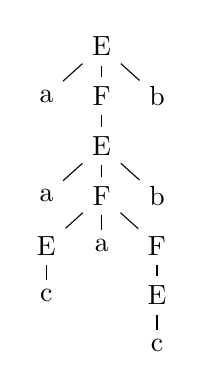
\begin{tikzpicture}[level distance=18pt,sibling distance=20pt,
   level 2/.style={sibling distance=20pt},
   level 3/.style={sibling distance=20pt},
]
\node {E}
 child {node {a} }
 child {node {F}
                child {node {E}
                       child { node {a} }     
                       child { node {F}
                               child { node {E} child {node {c}}}
                               child { node {a} }
                               child { node {F} child {node {E} child {node {c}}}}
                             }    
                       child { node {b} }     
                }
       }
 child {node {b} }
;
\end{tikzpicture}
}

\end{enumerate}

\item \begin{minipage}[t]{0.7\columnwidth}
 Build the LR(0) automaton for the following ambiguous grammar.
  \textbf{if}, \textbf{else}, and \textbf{null} are terminals; the
  third rule indicates $T$ may be the empty string.  Indicate the state
  in which the shift/reduce conflict appears.
\end{minipage}%
\begin{minipage}[t]{0.2\columnwidth}
\vspace{-0.8\baselineskip}
\ \
$
\begin{array}{l}
S' \rightarrow S \\
S \rightarrow \textbf{if}\ S\ T \\
S \rightarrow \textbf{null} \\
T \rightarrow \\
T \rightarrow \textbf{else}\ S
\end{array}
$
\end{minipage}

\def\pac{\ \cdot\ }
\newcommand{\id}{\textbf{Id}}

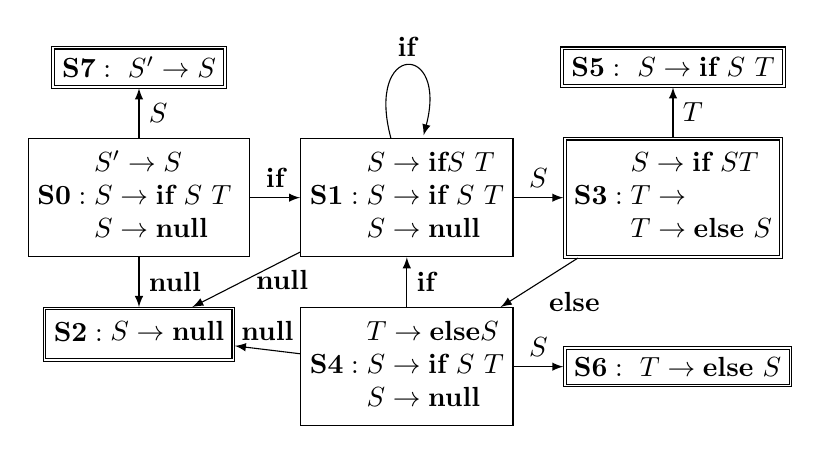
\begin{tikzpicture}[node distance=1.5pc]

  \node [draw] (S0) {$\textbf{S0}: \begin{array}{@{}l@{}}
    S' \rightarrow \pac S \\
    S \rightarrow \pac \textbf{if}\ S\ T\ \\
    S \rightarrow \pac \textbf{null} \\
  \end{array}$};

    \node [draw,right=of S0] (S1) {$\textbf{S1}: \begin{array}{@{}l@{}}
        S \rightarrow \textbf{if} \pac S\ T \\
        S \rightarrow \pac \textbf{if}\ S\ T \\
        S \rightarrow \pac \textbf{null}
      \end{array}$};

    \node [draw,accepting,above=of S0] (S7) {$\textbf{S7}:\ S'
      \rightarrow S \pac$};

    \node [draw,accepting,right=of S1] (S2) {$\textbf{S3}: \begin{array}{@{}l@{}}
        S \rightarrow \textbf{if}\ S \pac T \\
        T \rightarrow \pac \\
        T \rightarrow \pac \textbf{else}\ S
      \end{array}$};

    \node [draw,below=of S1] (S3) {$\textbf{S4}: \begin{array}{@{}l@{}}
        T \rightarrow \textbf{else} \pac S \\
        S \rightarrow \pac \textbf{if}\ S\ T \\
        S \rightarrow \pac \textbf{null}
      \end{array}$};

    \node [draw,accepting,below=of S0] (S4)
          {$\textbf{S2}: \begin{array}{@{}l@{}}
              S \rightarrow \textbf{null} \pac
            \end{array}$};

     \path [->]
     (S0) edge node [right] {$S$} (S7)
     (S0) edge node [above] {$\textbf{if}$} (S1)
     (S0) edge node [right] {$\textbf{null}$} (S4)
     ;
   
    \node [draw,accepting,right=of S3] (S5) {$\textbf{S6}:\ T
      \rightarrow \textbf{else}\ S \pac$};

    \path [->]
      (S3) edge node [right] {$\textbf{if}$} (S1)
      (S3) edge node [above] {$\textbf{null}$} (S4)
      (S3) edge node [above] {$S$} (S5);

    \node [draw,accepting, above=of S2] (S6)
          {$\textbf{S5}:\ S \rightarrow \textbf{if}\ S\ T \pac$};

    \path [->] (S1) edge node [above] {$S$} (S2)
               (S1) edge node [right] {$\textbf{null}$} (S4)
               (S1) edge [loop above] node [above] {$\textbf{if}$} ()
               (S2) edge node [right] {$T$} (S6)
               (S2) edge node [below right] {$\textbf{else}$} (S3);

\end{tikzpicture}

The shift/reduce conflict occurs in state S3 above: when the next
token is \textbf{else}, $T \rightarrow \pac \textbf{else}\ S$ 
indicates a shift; \textbf{else} is in the FOLLOW set of
$T$, indicating reduction by $T \rightarrow \pac$.

Ocamlyacc produces additional starting/ending states, but the state with the shift/reduce error is the same:

\begin{verbatim}
6: shift/reduce conflict (shift 7, reduce 3) on ELSE
state 6
        s : IF s . t  (1)
        t : .  (3)

        ELSE  shift 7
        $end  reduce 3
        t  goto 8
\end{verbatim}

Menhir's report is similar:

\begin{verbatim}
State 3:
s -> IF s . t [ ELSE # ]
-- On ELSE shift to state 4
-- On t shift to state 6
-- On ELSE reduce production t -> 
-- On # reduce production t -> 
** Conflict on ELSE
\end{verbatim}

\end{enumerate}
\end{document}
% Local Variables:
% compile-command: "pdflatex --halt-on-error hw2-solutions.tex"
% End:
